% compendium/portfolio-construction-risk/quant-strategy-structure.tex
% Entries migrated on 2026-10-15 from the legacy systematic-investing overview and alpha-models files (slice 30,
% sysinv/sysinvoverview.tex and sysinv/alphamod.tex), owned by the section overview portfolio-construction-risk, the
% files' map candidate. Dispositions and source checks in notes/migration-slices.md; the files verbatim in
% notes/artefacts/portfolio-construction-risk/systematic-investing-overview.tex and alpha-models.tex.

\section{The structure of a quant strategy and its alpha models}

\begin{qfdefinition}[Components of a quant trading strategy: alpha, risk and transaction cost models feeding portfolio construction, which interacts with execution, built on data and research]\label{def:quant-strategy-components}
\qffield{Statement} Narang's schematic of a live, production trading strategy has three modules, ``an alpha model, a risk model, and a transaction cost model'', which ``feed into a portfolio construction model, which in turn interacts with the execution model'' \citep[chap.~2, ``An Introduction to Quantitative Trading'', sec.~2.2, Exhibit~2.1, p.~17, page image]{s7-narang}:
\begin{itemize}
\item the \emph{alpha model} predicts the future of the instruments considered, to generate returns;
\item the \emph{risk model} helps limit exposure to factors ``unlikely to generate returns but could drive losses'', for example a trend follower's limit on directional exposure to commodities (pp.~17--18);
\item the \emph{transaction cost model} estimates the cost of the trades needed to move from the current to the desired portfolio (p.~18);
\item the \emph{portfolio construction model} balances profit, risk and cost to choose the best portfolio to hold; the difference between the target and the current portfolio is the list of trades (Exhibit~2.2, p.~18);
\item the \emph{execution model} carries out those trades, using inputs such as their urgency and the dynamics of liquidity, ``in an efficient and low-cost manner'' (p.~18).
\end{itemize}
The schematic covers only the production system; data, without which black boxes are ``inert and useless'', and research complete it (Exhibit~2.3, p.~19). Figure~\ref{fig:quant-strategy-structure} redraws Exhibit~2.1.
\begin{figure}[ht]
\centering
% compendium/portfolio-construction-risk/figures/strategystructure.tikz
% Moved from compendium/legacy/portfolio-construction-risk/figures/ in slice 30 (2026-10-15); the return arrow
% from execution to portfolio construction was added to match Narang's Exhibit 2.1. The original is kept verbatim
% in notes/artefacts/portfolio-construction-risk/systematic-investing-overview.tex.
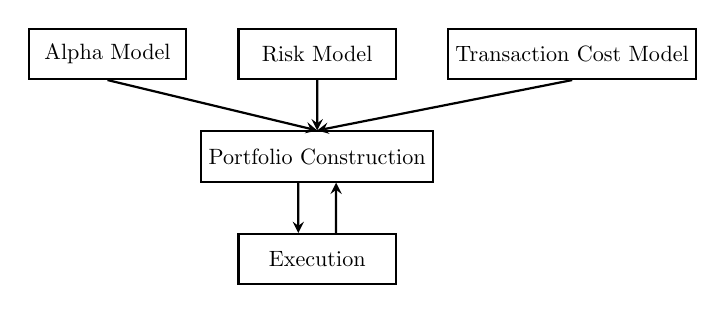
\begin{tikzpicture}[auto, thick, >=stealth, scale=0.8, transform shape]

    \usetikzlibrary{positioning}

    % Three modules arranged horizontally with reduced dimensions
    \node[draw, rectangle, minimum width=2.5cm, minimum height=0.8cm] (alpha) {Alpha Model};
    \node[draw, rectangle, minimum width=2.5cm, minimum height=0.8cm, right=0.8cm of alpha] (risk) {Risk Model};
    \node[draw, rectangle, minimum width=2.5cm, minimum height=0.8cm, right=0.8cm of risk] (tc) {Transaction Cost Model};

    % Portfolio Construction node directly below Risk Model
    \node[draw, rectangle, minimum width=2.5cm, minimum height=0.8cm, below=0.8cm of risk] (portfolio) {Portfolio Construction};

    % Execution node below Portfolio Construction
    \node[draw, rectangle, minimum width=2.5cm, minimum height=0.8cm, below=0.8cm of portfolio] (execution) {Execution};

    % Arrows connecting the nodes
    \draw[->] (alpha.south) -- (portfolio.north);
    \draw[->] (risk.south) -- (portfolio.north);
    \draw[->] (tc.south) -- (portfolio.north);
    % Narang's Exhibit 2.1 (p. 17) shows the two modules interacting: an arrow down and one back up.
    \draw[->] ([xshift=-0.3cm]portfolio.south) -- ([xshift=-0.3cm]execution.north);
    \draw[->] ([xshift=0.3cm]execution.north) -- ([xshift=0.3cm]portfolio.south);
    
\end{tikzpicture}



\caption{The modules of a live quant trading strategy, after Narang's Exhibit~2.1 (p.~17); data and research, his Exhibit~2.3, are not drawn.}\label{fig:quant-strategy-structure}
\end{figure}

\qffield{Conditions} Narang calls a trader a quant when both what to own and how much are decided systematically as standard practice, allowing emergency overrides (sec.~2.1, p.~16). The structure ``is by no means universal'': many strategies run without a transaction cost, portfolio construction or execution model, risk constraints can be built into the alpha model, and some links are recursive, such as executions feeding the cost model (p.~19).

\qffield{Practice} Each module has its entries: forecasts in \hyperref[def:alpha-model-taxonomy]{alpha models} and \hyperref[meth:alpha-strategy-specification]{their specification}, combined in \hyperref[meth:alpha-signal-combination]{signal combination}; risk in \hyperref[mod:factor-risk-model]{the factor risk model}; costs in \hyperref[mod:portfolio-transaction-cost-function]{cost functions}; the decision in \hyperref[meth:rule-based-position-sizing]{rule-based sizing} and \hyperref[mod:mean-variance-portfolio-optimisation]{mean--variance optimisation}; execution in \hyperref[def:order-exposure-decisions]{order exposure decisions}; and the research and production chain around them in \hyperref[meth:strategy-production-lifecycle]{the strategy production lifecycle}. Checked: Narang's Exhibit~2.2 trades follow from target minus current weights ($-25-(-30)=+5$, $25-20=+5$, $25-40=-15$, $-25-(-10)=-15$ percent).

\qffield{Pitfalls} The legacy diagram drew only a downward arrow from portfolio construction to execution; Narang's exhibit and text show the two interacting, and the redrawn figure adds the return arrow. The legacy description of the risk model as ``directional exposure limit on an asset class'' generalises his single example. As in \hyperref[mod:factor-risk-model]{the factor risk model}, the risk model informs the decision; the portfolio construction model selects and sizes.

\qffield{See also} \hyperref[def:quant-strategy-risk-sources]{sources of strategy risk} (model risk can arise in every module); \hyperref[meth:quant-strategy-monitoring]{strategy monitoring}.

\qffield{Further reading} The legacy overview, its chapter wrapper and its original diagram are kept verbatim in the section's folder of \nolinkurl{notes/artefacts/}, as\\ \nolinkurl{systematic-investing-overview.tex}.

\qffield{Index} quant trading system; black box; alpha model; risk model; transaction cost model; portfolio construction model; execution model; target portfolio; trade list; data; research; production system

\qffield{Status} Verification: partly checked 2026-10-15 (against the text layer of a local copy of \texttt{s7-narang}, third edition, Wiley 2024, chap.~2, secs.~2.1--2.2, pp.~16--19, with Exhibit~2.1 on p.~17 by page image; Exhibit~2.2 arithmetic checked). Stability: draft. Currency: practitioner framework as of 2024.
\end{qfdefinition}

\begin{qfdefinition}[Alpha models: theory-driven and data-driven, and Narang's eight classes of theory-driven alpha by input]\label{def:alpha-model-taxonomy}
\qffield{Statement} Narang defines alpha, ``not conventional'' by his own account, as ``skill in timing the selection and/or sizing of portfolio holdings''; an alpha model is the software that does this timing systematically \citep[chap.~3, ``Alpha Models: How Quants Make Money'', pp.~23--24]{s7-narang}. Alpha models are \emph{theory-driven}, starting from an economic explanation that is then tested, or \emph{data-driven}, looking for patterns without a prior theory (sec.~3.1, pp.~25--28). Theory-driven alphas fall into eight classes, sorted by input (Exhibit~3.2, p.~29):
\begin{itemize}
\item \emph{price data}: \emph{trend} or momentum, explained by slow consensus-building or by ``greater fools'' (pp.~29--30); \emph{mean reversion}, explained by temporary liquidity imbalances, such as index additions, and overshooting, with statistical arbitrage on similar stocks as its best-known form (pp.~33--35); and \emph{technical sentiment}, from option volumes and skews, trading volume and the order book (pp.~35--37);
\item \emph{fundamental data}: \emph{value/yield}, ratios with price in the denominator such as earnings yield, read as being paid to hold riskier instruments (pp.~38--41); \emph{growth/sentiment}, including analysts' revisions (pp.~42--43); \emph{supply/demand} (pp.~43--44); \emph{quality}, from leverage, revenue diversity, management, fraud risk and quality sentiment (pp.~44--46); and \emph{tactical/events}, one-off events such as elections or the pandemic (pp.~46--47).
\end{itemize}
Data-driven strategies are ``far less widely practiced'', more common at high frequency where data are abundant, and in his view mostly unsuccessful as forecasters of markets (sec.~3.3, pp.~47--52).

\qffield{Conditions} The classes are Narang's framework for organising strategies, not a result: he offers explanations for trend and reversion and cites little evidence: two papers for value/yield (Fama and French, n.~5; Ball, n.~6; pp.~37--40) and his reading of research on volume as a contrarian signal (p.~37), and otherwise examples and anecdotes. Trend and reversion coexist ``largely'' because they operate at different horizons, longer trends with shorter oscillations (Exhibit~3.5, pp.~35--36). He stresses that every class has ``relatively long periods of poor returns'' because the behaviours are ``unstable and episodic'' (p.~32), and that some strategies once called alpha, such as longer-term trend, are now treated by many as risk premia or ``smart beta'' (p.~24).

\qffield{Practice} Interpretation: whether a class is used as an alpha to forecast, a premium to harvest or a risk to limit depends on the strategy, as in \hyperref[mod:factor-risk-model]{the factor risk model}. His relative-value example combines value and financing: ``when done on a relative basis \dots\ this strategy is also known as a carry trade'', earning the yield spread (p.~40); with the euro at 4.25 percent and the dollar at 2 percent, the carry is 2.25 percent (checked).

\emph{Published evidence for four of the classes} (third batch of 2026-10-17).
\begin{itemize}
\item \emph{Carry is not value.} Koijen, Moskowitz, Pedersen and Vrugt define an asset's carry as ``its expected return assuming that its price does not change'', measurable in advance without a pricing model \citep[NBER WP 19325, August 2013, abstract and sec.~I, PDF pp.~2--3]{alpha-carry}. Carry predicts returns in the cross-section and over time in global equities, bonds, currencies, commodities, Treasuries, credit and index options. A carry strategy within an asset class earns an annualised Sharpe ratio of 0.7 on average, and one diversified across classes 1.1 (p.~2). Regressed on value, momentum and time-series momentum factors, carry keeps a significant alpha in every class. Equity carry loads positively on value without much loss of alpha. Commodity carry loads negatively on value and positively on momentum, and its alpha falls by 29 to 64 basis points a month, still significant. Currency and credit carry show no reliable loading (Table~IV discussion, pp.~23--24). So Narang's ``carry trade'' for relative value is a distinct signal from value, though correlated with it in places.
\item \emph{Value.} Asness, Moskowitz and Pedersen find ``consistent value and momentum return premia across eight diverse markets and asset classes''. Value and momentum are negatively correlated with each other, within and across classes, and are partly linked to global funding liquidity risk \citep[abstract, p.~929]{alpha-value}.
\item \emph{Quality and growth.} Asness, Frazzini and Pedersen define quality as characteristics investors should pay more for: profitability, growth and safety, with payout. A quality-minus-junk factor ``earns significant risk-adjusted returns in the United States and across 24 countries'', while high-quality stocks trade at only modestly higher prices \citep[published version, abstract, p.~34]{alpha-qmj}. Growth enters as one component of quality, not as a separate premium; the paper gives no evidence for a stand-alone growth premium.
\item \emph{Mean reversion in residuals.} Avellaneda and Lee trade mean reversion in stock residuals from PCA or sector-ETF factor models, assuming 5 basis points a trade. PCA strategies earn an annual Sharpe ratio of 1.44 over 1997--2007, but only 0.9 in 2003--2007; ETF strategies 1.1, with the same decline after 2002. Their August 2007 results agree with Khandani and Lo's unwinding account \citep[version of 15 June 2009, abstract and sec.~1, pp.~1 and~4]{alpha-residual}. \emph{The trading rule} (fourth batch of 2026-10-17): the residual's distance from its fitted Ornstein--Uhlenbeck mean in equilibrium standard deviations is the \emph{s-score}, $s_i=(X_i(t)-m_i)/\sigma_{\mathrm{eq},i}$; they open a trade when $|s_i|>1.25$, close longs when $s_i>-0.50$ and shorts when $s_i<0.75$ (eqs.~(15)--(16), pp.~18--19). The cutoffs were ``selected \dots\ empirically, based on simulating strategies from 2000 to 2004'', and the asymmetric short exit from 2000--2002, inside the 1997--2007 backtest period, so the reported Sharpe ratios include an in-sample choice of thresholds (p.~19). \emph{Where contrarian profits come from.} For the Lo--MacKinlay rule, which weights each stock by minus its lagged return relative to the equal-weighted market, expected profit splits into a cross-autocovariance term, an own-autocovariance term and the cross-sectional variance of mean returns. On 551 NYSE--AMEX stocks with complete weekly returns from 6 July 1962 to 31 December 1987, half the lag-1 expected profit comes from positive cross-autocovariances, about 67 percent in the central size quintile; they conclude that ``less than 50 percent of the expected profits from a contrarian investment rule may be attributed to overreaction'', with larger stocks leading smaller ones \citep[NBER WP~2977, May 1989, sec.~4, printed p.~17, and sec.~6, printed p.~22]{wide-lo-mackinlay-contrarian}. So residual reversal is partly a lead--lag effect, which a factor-residual construction may remove or keep depending on the factors. Gatev, Goetzmann and Rouwenhorst's distance-based pairs, 1962--1997, earn about 12 percent a year in excess for top pairs, ``reduced---but still positive and significant'' after bid--ask bounce and costs \citep[NBER WP 7032, 1999, sec.~I, p.~1]{alpha-gatev}.
\end{itemize}
Fama and French (1993) was not read for this batch.

\qffield{Pitfalls} The legacy block listed five classes (trend, mean reversion, value/yield, growth, quality); the third edition has eight, adding technical sentiment, supply/demand and tactical/events. The legacy sentence that a moving-average crossover ``has less than one point of return for every point of downside risk'' attaches to one rule what Narang says of ``the typical successful trend follower'' (p.~32), with no data. \emph{Evidence} (batch of 2026-10-17). Moskowitz, Ooi and Pedersen find ``significant `time series momentum' in equity index, currency, commodity, and bond futures for each of the 58 liquid instruments'', with persistence over one to 12 months that partly reverses later. Their diversified portfolio ``performs best during extreme markets'' \citep[abstract, p.~228]{s6-tsmom}. Each position is sized to an ex ante annualised volatility of 40 percent, $40\%/s_{t-1}$, where $s^2_t=261\sum_i(1-\delta)\delta^i(r_{t-1-i}-\bar r_t)^2$ is an exponentially weighted variance of daily returns with centre of mass $\delta/(1-\delta)=60$ days, the same for all assets, and the estimate at $t-1$ is applied to returns at $t$ to avoid look-ahead; the 40 percent is ``inconsequential'' and makes the equal-weighted factor about 12 percent volatile over 1985--2009 \citep[secs.~2.4 and~4.1, eq.~(1), pp.~233 and~236]{s6-tsmom} (fourth batch of 2026-10-17). Hurst, Ooi and Pedersen extend an equal-weighted 1-, 3- and 12-month version, scaled to 10 percent ex ante volatility, to 67 markets from January 1880 to December 2016 \citep[reprint PDF pp.~3--7, Exhibit~1 on PDF p.~4]{alpha-century}:
\begin{itemize}
\item excess returns of 18.0 percent a year gross, 11.0 percent net of simulated costs, and 7.3 percent net of costs and a hypothetical 2-and-20 fee, at 9.7 percent volatility, a net Sharpe ratio of 0.76;
\item positive net returns in every decade (lowest 1.6 percent, 1910--1919), and positive returns in 8 of the 10 largest drawdowns of a 60/40 portfolio;
\item its own drawdowns ``losing up to 25\%''.
\end{itemize}
Against Narang's sentence, a net 7.3 percent a year over a worst drawdown of about 25 percent is roughly 0.3 points of annual return per point of maximum drawdown (Interpretation; drawdown read from the text, not Exhibit~8's table). That is consistent with ``less than one point'' on that measure, while the volatility-based ratio is 0.76. Both papers are by AQR principals and are simulated, before any real fund's frictions beyond the cost and fee assumptions. The 2017 article read is a copy on a Yale course page, a journal reprint whose hosting is not the publisher's. The legacy ``buying undervalued security and selling overvalued security is a carry trade'' drops the context of his sentence, in which ``this strategy'' is the yield strategy, so that the long earns the higher yield; interpretation, not checked against the factor readings: value (cheapness against fundamentals) and carry (the return if prices do not change) are distinct signals in later work, though they can coincide. His performance figures for Seykota, Mint and Renaissance (pp.~31--32) are anecdotes with press or web sources. ``In general, strategies that use data-mining techniques to forecast markets do not work'' (p.~49) is his judgement. Evidence for each class belongs to its specialist pathway (stubs in the overview's note).

\qffield{See also} \hyperref[meth:alpha-strategy-specification]{alpha strategy specification}; \hyperref[meth:alpha-signal-combination]{signal combination}; \hyperref[meth:hypothesis-driven-strategy-research]{hypothesis-driven strategy research} (theory-driven research as a method); \hyperref[pit:parameter-overfitting]{parameter overfitting}.

\qffield{Further reading} The legacy file, verbatim, is in \nolinkurl{alpha-models.tex} in the section's folder of \nolinkurl{notes/artefacts/}.

\qffield{Index} alpha; alpha model; theory-driven; data-driven; data mining; trend following; momentum; mean reversion; statistical arbitrage; technical sentiment; value; yield; earnings yield; carry; quant long/short; growth; estimate revisions; supply and demand; quality; tactical events; smart beta; risk premia

\qffield{Status} Verification: partly checked 2026-10-15 (against the text layer of a local copy of \texttt{s7-narang}, third edition, Wiley 2024, chap.~3, secs.~3.1--3.3, pp.~23--52, with Exhibit~3.2 on p.~29 by page image; the carry example checked; batch of 2026-10-17: \texttt{s6-tsmom}, author-hosted journal copy, abstract; \texttt{alpha-century}, \emph{JPM} Fall 2017 reprint, PDF pp.~3--7 with Exhibit~1 by page image; fourth batch of 2026-10-17: Lo and MacKinlay (NBER WP~2977), Avellaneda and Lee's eqs.~(15)--(16) and Moskowitz, Ooi and Pedersen's secs.~2.4 and~4.1). Stability: draft. Currency: practitioner taxonomy as of 2024; anecdotes from 1970 to 2023.
\end{qfdefinition}

\begin{qfmethod}[Specifying an alpha strategy: forecast target, time horizon, bet structure, investment universe, model specification, conditioning variables and run frequency]\label{meth:alpha-strategy-specification}
\qffield{Statement} Narang lists the choices that turn an alpha idea into a strategy \citep[chap.~3, sec.~3.4, pp.~52--63]{s7-narang}:
\begin{enumerate}
\item \emph{forecast target}: direction, magnitude and/or duration of a move, possibly with a confidence. Signal strength is the expected return and/or the confidence, and ``in general, though certainly not always'' a stronger signal means a bigger bet (pp.~52--53);
\item \emph{time horizon}, from microseconds to a year or more, with his classes high-frequency, short-term (a day to two weeks), medium-term and long-term (pp.~53--55);
\item \emph{bet structure}: an instrument by itself (intrinsic) or relative to others, in pairs or larger clusters, grouped statistically or heuristically (pp.~55--57);
\item \emph{investment universe}: geography, asset class, instrument class and exclusions, preferring liquidity, plentiful clean data and predictable behaviour (pp.~57--59);
\item \emph{model specification}: the precise definition and parameters, and how often the model is refitted (pp.~59--60);
\item \emph{conditioning variables}: modifying conditioners such as stops and profit targets, and secondary conditioners that require agreement between signals (pp.~60--61);
\item \emph{run frequency}: from monthly to continuous, trading noise and cost against large, market-moving rebalances and missed prices (pp.~61--62).
\end{enumerate}
With two forecast types, four horizons, two bet structures and four asset classes, one idea gives $2\times4\times2\times4=64$ variants (pp.~62--63; checked).

\qffield{Conditions} Narang qualifies several items himself. Very large signals are rare, so the forecast--outcome relation may be less reliable there (p.~53). Differences between strategies are larger at short horizons, because small changes are amplified over many trades (pp.~54--55). Pairs are rarely precisely comparable, statistical groupings ``can be fooled by the data'' and heuristic ones are imprecise and rigid; grouping techniques suffer when regimes change (pp.~56--57). Refitting raises the risk of overfitting (p.~60). Most directional trend-following strategies make money on a minority of their trades, ``often less than 40 percent'' (pp.~60--61).

\qffield{Practice} Interpretation: forecast strength becomes position size only through calibration and the portfolio decision. Sizing by strength presumes that strength is calibrated to realised returns (rank-based or equal sizing need not); size also depends on each instrument's risk, its correlation with other positions, costs and constraints, so ``bigger signal, bigger bet'' holds for a calibrated forecast with other inputs equal (\hyperref[meth:rule-based-position-sizing]{rule-based sizing}, where Narang gives the case against unequal weights; \hyperref[mod:mean-variance-portfolio-optimisation]{mean--variance optimisation}; \hyperref[mod:portfolio-transaction-cost-function]{cost functions}). Specification choices made after looking at results are trials to be counted (\hyperref[pit:parameter-overfitting]{parameter overfitting}).

\qffield{Pitfalls} ``Relative alpha strategies tend to exhibit smoother returns during normal times than intrinsic alpha strategies, but \dots\ unique problems related to incorrect groupings during stressful periods'' (p.~57) is a conditional generalisation with no data in the chapter; the legacy kept it. Narang's statement that machine-learning techniques are ``designed to provide'' a ``scientifically valid way of testing \dots\ without overfitting'' (p.~60) is not adopted. Interpretation: searching many specifications is a source of overfitting, which no technique removes by its name (\hyperref[meth:backtest-evaluation-diagnostics]{backtest diagnostics}). His biotech example is that ``some quants exclude'' such stocks (p.~58), which the legacy turned into a rule. The legacy omitted the conditioning variables. ``Relative value'', he notes, is industry jargon for any relative bet structure, mostly unrelated to value (p.~57).

\qffield{See also} \hyperref[def:alpha-model-taxonomy]{alpha models}; \hyperref[meth:alpha-signal-combination]{signal combination}; \hyperref[meth:hypothesis-driven-strategy-research]{hypothesis-driven strategy research}; \hyperref[mod:factor-risk-model]{factor risk model} (relative bets as risk control).

\qffield{Further reading} The legacy file, verbatim, is in \nolinkurl{alpha-models.tex} in the section's folder of \nolinkurl{notes/artefacts/}.

\qffield{Index} forecast target; signal strength; confidence; time horizon; high-frequency; short-term; medium-term; long-term; bet structure; intrinsic; relative; pairs; clusters; grouping; relative value; investment universe; liquidity; model specification; parameters; refitting; conditioning variables; stop-loss; profit target; time stop; run frequency

\qffield{Status} Verification: partly checked 2026-10-15 (against the text layer of a local copy of \texttt{s7-narang}, third edition, Wiley 2024, chap.~3, sec.~3.4, pp.~52--63, with Exhibits~3.7 and~3.8 read from the text layer; the permutation count checked). Stability: draft. Currency: practitioner account as of 2024.
\end{qfmethod}
